\chapter{基础知识}
\label{chap:preliminary}

\textit{}s

\textit{本章介绍本文研究所需的信息论、博弈论及隐私保护的基本概念,包括Shannon信息论及其扩展,策略博弈、扩展博弈等博弈论概念,隐私分类及隐私保护基本模型。本章的内容主要为后文展开具体研究奠定基础。}
\section{Shannon信息论及其扩展}

\subsection{信息通信模型}
信息论\cite{shannon1948mathematical,
	stone2018information}是信息科学的基本工具,信息论对于量化信息的不确定性和信息量有重要的作用。信息通信模型最早由Shannon在其《通信的数学原理》论文中提出,如图\ref{fig:communication-model}所示。

\begin{figure}[htbp]
	\centering
	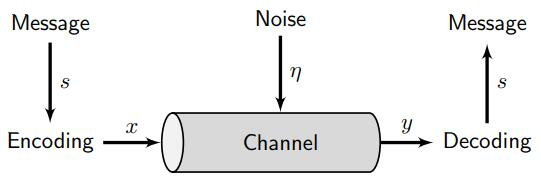
\includegraphics[width = 0.6\linewidth]{./figures/shannon-communicaiton-model.jpg}
	\caption{信息通信模型\cite{stone2018information}.
	}
	\label{fig:communication-model}
\end{figure}

信息通信模型\cite{stone2018information}由信源消息、编码器、信道、解码器、信宿消息和噪音构成,信源消息(数据)在作为信道输入之前被编码器进行编码;编码后的信源消息在信道中传输,传输过程中会受到噪声影响;解码器从信道中接收到加噪后的信息,解码为信宿消息。Shannon定义的上述通信模型可以描述任何人造或自然的系统间的通信信息量。对任意额通信系统,都有:1)信道容量,即可以被信道传输信息的最大量;2)极限受损。即信道中最大的噪音量;3)通过编码,可以达到这两个极限。



\subsection{信息熵}


\begin{definition}
	对于事件集中的某一特定事件$x$,$x$的概率为$p(x)$,则$x$的香农信息为$-\text{log}p(x)$。
\end{definition}
上述定义通常被称为自信息,其表示该事件发生了所需要传递的信息的比特数量。而熵表示自信息的平均量,即某一个随机事件变量的所有事件取值发生时,该随机变量的平均Shannon信息量,即

\begin{definition}
随机变量$X=(x_1,x_2,...,x_n)$,其概率分布为~$\{p(x_1),p(x_2),....,p(x_n)\}$~,则该随机变量的熵为
\begin{equation}
H(x)=-\sum_{i=1}^{n}p(x_i)log_2p(x_i)
\end{equation}
\end{definition}
在Shannon通信模型中,信源产生的随机事件的熵称为信源熵,信宿产生的随机事件的熵称为信宿熵。信源熵是信源消息变量~$X$~可以表示的平均信息比特数,即平均信息量。但是,上述定义给出的熵是离散变量的熵,对于连续熵的定义,本文不再讨论,可参考文献\cite{stone2018information}。

熵是对不确定度的一种度量,当不确定下降时,我们得到了信息,因此信息和熵是一体两面的。上述定义的熵是针对所有离散随机变量的,任意随机变量都存在一个概率分布,使得该随机变量的熵为最大,该分布称为最大熵分布。通过熵的定义可知,当$n$个随机事件均匀分布时,该随机变量熵最大,即有

\begin{equation}
H(x)_{Max}=-n\sum_{i=1}^{n}p(x_i)log_2p(1/n)
\end{equation}


针对Shannon通信模型,若在信源输入消息,则会对信宿消息的不确定度产生影响,从平均意义上就有平均不确定度的影响,即条件熵。

\begin{definition}
	随机变量$X=(x_1,x_2,...,x_n)$是输入,其概率分布为~$\{p(x_1),p(x_2),....,p(x_n)\}$~,随机变量$Y=(y_1,y_2,...,y_n)$是输出,其概率分布为~$\{p(y_1),p(y_2),....,p(y_m)\}$~,则输入$X$时,$Y$的不确定度为
	\begin{equation}
	H(Y/x)=-\sum_{i=1}^{n}-\sum_{j=1}^{m}p(y_j/x_i)log_2p(y_j/x_i)
	\end{equation}
\end{definition}


\subsection{互信息}
变量$X$与$Y$之间的互信息$I(X,Y)$是指,输入$X$时的每个随机事件能够提供给$Y$的平均信息量,互信息可以表示为

\begin{equation}
I(X,Y)=H(X)-H(X/Y)=H(Y)-H(Y/X)
\end{equation}

\subsection{结构信息论}

\section{博弈论}
博弈论\cite{owen2001,gibbons1992} 是一个自我利益实体(即博弈者)之间相互作用的数学模型,它总是用于为这些实体寻找冲突与合作的解决方案。 博弈包含实体之间的迭代,并且每个博弈者在每次迭代中都将执行一个操作。 最后,博弈达到了解决方案(即平衡),所有博弈者都获得了自己最大的收益。 在特定的博弈中,博弈者是理性的,这意味着每个博弈者都会采取行动来响应他人的行动,以获取最大的利益。

有一些术语用来描述博弈、博弈者、行为、回报、策略和均衡\cite{liang2013}。博弈者是参与底层博弈的实体,博弈者可以是人、机构或信息系统;动作是每个博弈者在博弈的每个迭代中所做的动作,每个博弈者都知道每个其他博弈者的所有可选动作;博弈者的回报是对于他在博弈中采取的行动的返回值;博弈者的策略是他/她的行动计划,该计划根据他/她对行动历史的了解来指定要采取的行动。策略可以是纯策略,也可以是混合策略;均衡是一个博弈的解,是所有博弈者各自获得最大利益的策略组合。博弈论在信息安全和隐私保护的许多领域都得到了应用,详见\cite{liang2013,tian2019}。
\subsection{博弈模型}
\subsection{策略博弈}
\subsection{扩展博弈}
\subsection{演化博弈}


\section{隐私定义及隐私保护}
\subsection{身份隐私}
\subsection{属性隐私}
\subsection{隐私保护模型}

